\section{1-Wire protokol}
%https://www.maximintegrated.com/en/products/digital/one-wire.html
Sensoren benytter en 1-Wire forbindelse til at kommunikere med mikroprocessoren. 1-Wire er en teknologi hvor en  enkelt serial forbindelse fungere som data forbindelse i begge retninger. 

Dette gøres ved at forbinde dataforbindelsen på sensoren med mikroprocessoren, og en pull-up modstand forbundes til 5 V som det ses på figur \ref{one_wire_schematic}. 


\begin{figure}[h!]
  \centering
  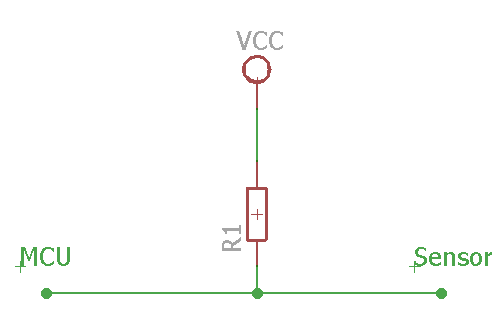
\includegraphics[width=0.8\textwidth]{figures/onewire_eksempel.png}
  \caption{1-Wire data forbindelse mellem sensor og mikroprocessor}
  \label{one_wire_schematic}
\end{figure}

1-Wire fungere lidt anderledes end en normal data forbindelse. Data bliver læst som tiden hvor der er et 0 V signal, og pull-op modstanden vil så trække signalet høj hver gang der intet signal er. Der vil ligge 5 V på dataforbindelsen indtil enten sensor eller mikroprocessor begynder at sende 0 V, hvor den anden enhed så kan registrer hvor længe der ligge 0 V på dataforbindelsen. Tidslængden af 0 V signalet afgører om den enheder der modtager skal opfatte signalet som et 0 eller 1. Hvis der skal skrives et 0 udsendes der et 0 V signal i 60 $\mu$S og hvis der skal skrives 1 sendes der 0 V i 15 $\mu$S. 

Når der skal læses over 1-Wire sker dette 30 $\mu$S efter at der er registreret en falded spænding. Dette vil så sige at da 0 svare til et delay på 60 $\mu$S vil der måles 0 V her, og da 1 svare til et delay på maksimum 15 $\mu$S vil der læses 5 V eller et højt signal her.


\begin{figure}[h!]
  \centering
  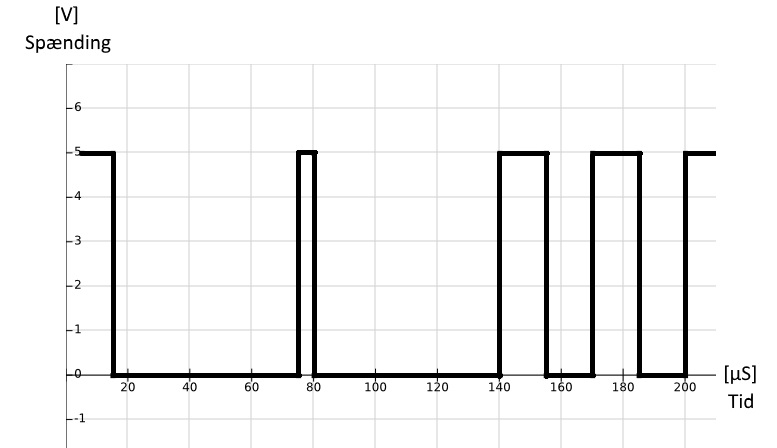
\includegraphics[width=0.8\textwidth]{figures/onewire.png}
  \caption{1-Wire graf der viser hvad der ligger på dataforbindelsen når der bliver skrevet.}
  \label{onewire_graph}
\end{figure}

På figur \ref{onewire_graph} ses det hvordan det vil se ud hvis man ønsker at sende et 0xC over 1-Wire forbindelsen. Det binære tal for 0xC er 1100 og da 1-Wire skriver fra LSB\footnote{Least Significant Bit}, skal det ses bagfra. Dette ses på grafen som 2 "store" mellemrum hvor der bliver skrevet 0 V på dataforbindelsen efterfuldt af to "korte" som svare til to 1 tal. Dette er blevet eftermålt med et oscilloskop og kan ses på figur \ref{SCR01}.


\begin{figure}[h!]
  \centering
  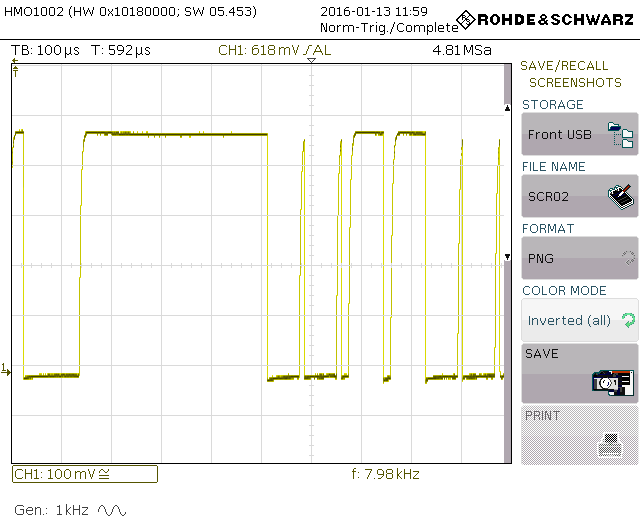
\includegraphics[width=0.8\textwidth]{figures/SCR02.png}
  \caption{Måling af 1-Wire data forbindelse med et oscilloskop.}
  \label{SCR02}
\end{figure}

Figuren viser hvad der måles på dataforbindelsen når mikroprocessoren skriver SKIPROM kommandoen til sensoren.
Fra ca. midten af figuren ses det SKIPROM funktionen som består af 0xCC eller 1100 1100 i binær. Starten af 1100 (læst fra LSB) ses på i midten af grafen.